\mode*

\section{Just nu}

\begin{frame}
  \begin{question}[Situationen ju nu]
    \begin{itemize}
      \item Utifrån det ni har läst.
      \item Hur upplever ni er situation just nu?
    \end{itemize}
  \end{question}

  \begin{exercise}
    \begin{itemize}
      \item Breakout rooms, 3 personer, 10 minuter.
    \end{itemize}
  \end{exercise}
\end{frame}

\begin{frame}
  \begin{question}
    \begin{itemize}
      \item Vad fanns det för olika teman i diskussionerna?
      \item Ergonomi, stress eller ohälsa?
    \end{itemize}
  \end{question}
\end{frame}


\section{I allmänhet}

\begin{frame}
  \begin{question}
    \begin{itemize}
      \item Vad gör er stressade?
      \item Vad gör ni för att hantera det?
    \end{itemize}
  \end{question}

  \begin{exercise}
    \begin{itemize}
      \item Breakout rooms, 3 personer, 10 minuter.
    \end{itemize}
  \end{exercise}
\end{frame}


\section{Framtiden}

\begin{frame}
  \begin{question}
    \begin{itemize}
      \item Vad kan KTH göra för att minska negativ stress?
    \end{itemize}
  \end{question}

  \begin{exercise}
    \begin{itemize}
      \item Breakout rooms, 3 personer, 10 minuter.
    \end{itemize}
  \end{exercise}
\end{frame}

\begin{frame}
  \begin{question}
    \begin{itemize}
      \item Hur kan man ändra kurserna ni läst för att underlätta?
      \item Vilken kurs är den största \enquote{syndaren}?
    \end{itemize}
  \end{question}

  \begin{exercise}
    \begin{itemize}
      \item Breakout rooms, 3 personer, 10 minuter.
    \end{itemize}
  \end{exercise}
\end{frame}

\begin{frame}
  \begin{figure}
    
\includegraphics[height=0.8\textheight]{betygshets.png}
    \caption{\url{https://www.forskning.se/2021/09/02/betygshets-i-skolan-ger-elever-okad-stress-och-ohalsa/}}
  \end{figure}
\end{frame}

\begin{frame}
  \begin{figure}
    
\includegraphics[height=0.8\textheight]{grading-scales.png}
    \caption{\url{https://journals.lww.com/academicmedicine/fulltext/2011/11000/Relationship_of_Pass_Fail_Grading_and_Curriculum.29.aspx}}
  \end{figure}
\end{frame}

\begin{frame}
  \begin{figure}
    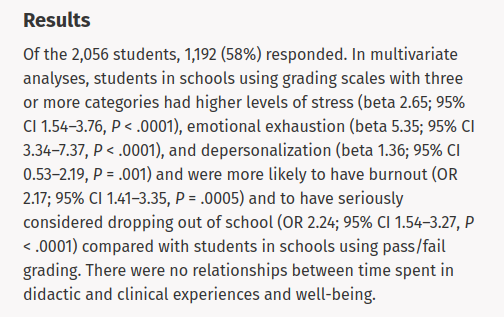
\includegraphics[height=0.8\textheight]{grading-results.png}
    \caption{\url{https://journals.lww.com/academicmedicine/fulltext/2011/11000/Relationship_of_Pass_Fail_Grading_and_Curriculum.29.aspx}}
  \end{figure}
\end{frame}

\begin{frame}
  \begin{question}
    \begin{itemize}
      \item Om vi ändrar alla kurser till P/F.
      \item Hur skulle det påverka erat beteende?
    \end{itemize}
  \end{question}

  \begin{exercise}
    \begin{itemize}
      \item Breakout rooms, 3 personer, 10 minuter.
    \end{itemize}
  \end{exercise}
\end{frame}


